\documentclass{standalone}
\usepackage{tikz}

\begin{document}
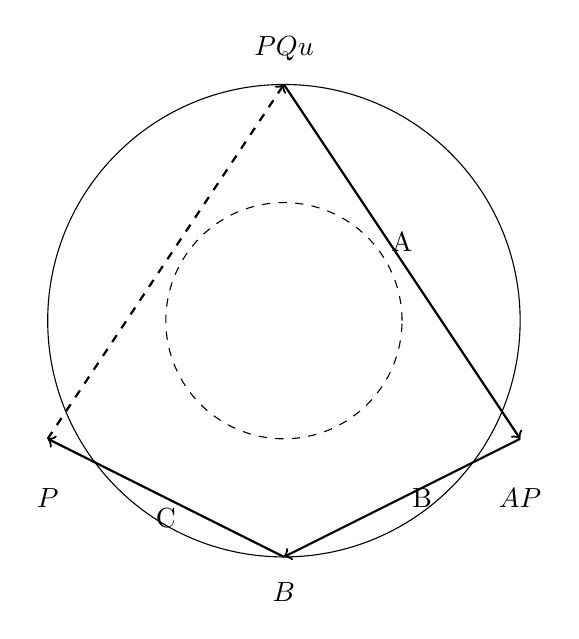
\begin{tikzpicture}[scale=1.5]
    % Draw the outer circle
    \draw (0,0) circle (2cm);
    
    % Draw the inner circle
    \draw[dashed] (0,0) circle (1cm);
    
    % Label the regions
    \node at (0,2.3) {$PQu$};
    \node at (-2,-1.5) {$P$};
    \node at (2,-1.5) {$AP$};
    \node at (0,-2.3) {$B$};
    
    % Draw the arrows
    \draw[->, thick] (0,2) -- node[midway, above] {A} (2,-1);
    \draw[->, thick] (2,-1) -- node[midway, right] {B} (0,-2);
    \draw[->, thick] (0,-2) -- node[midway, below] {C} (-2,-1);
    
    % Connect back to the start
    \draw[->, thick, dashed] (-2,-1) -- (0,2);
\end{tikzpicture}
\end{document}